\chapter{Literature Review}\label{chap_lit_review}

This chapter contains concepts and equations necessary for the work presented. The chapter begins by defining a sound wave in terms of physics and then in terms of signal processing, some spectral features are defined in both theory and algorithm. This is followed by an introduction to dynamical systems and bifurcation theory describing the type of bifurcations. The final section of this chapter is concern with defining nonlinear optimization and describing the necessary concepts.

\section{Waves}\label{subsec_waves}

In fluid dynamics a wave is defined as the propagation of a perturbation of one or more physical variables, usually periodic and some times having a well defined frequency (periodic motions), which is created by the vibration of an object, called source of vibration. When the wave is in motion is called a \textit{traveling wave}, while a \textit{stationary wave} is a wave such that it remains in a constant position. Waves can overlap, they can combine to make constructive or destructive interference.\\

When the wave moves in a medium it is a \textit{mechanical wave}, while when it does not require a medium to travel through it is an \textit{electromagnetic wave}, propagating through vacuum (like light). Another classification has to do with the direction of the motion and vibration. A \textit{longitudinal wave} has the same direction of vibration as the direction traveling, while a \textit{transverse wave} moves perpendicular to the direction of oscillation.\\


Using differential calculus the most general equation that a wave, regardless of the type or nature of the wave, satisfies is a linear second-order partial differential equation
which, in the most general case, can be  a forcing\footnote{the right-hand side represents a non-homogeneity function that acts as source of oscillations $(f(t,\vec{r}))$, it is often called the forcing or driving function} equation
\begin{gather}\label{general_wave_equation}
    \frac{1}{v^2}\frac{\partial^2x(t,\vec{r})}{\partial^2 t^2} -  \nabla^2 x(t,\vec{r})  = f(t,\vec{r})
\end{gather}

where $v=||\vec{v}||$ is the magnitude of the sound speed, $x(t,\vec{r})$ the amplitude of the wave, and $\vec{r}$ the vector position. A particular solution is any \textit{traveling wave}, a space and time depending function satisfying $x(x,t) = x(\vec{r}\pm \vec{c}t)$, or even a linear combination of them, since the wave equation is a linear hence satisfies the superposition principle. \cite{book_birdsongs}. The backward (or leftward) wave is $x(\vec{r}+ \vec{c}t)$, while $x(\vec{r}-\vec{c}t)$ represents a forward (or rightward) wave.

The energy transport by the wave is related to their frequency and amplitude.

\subsection{Sound Waves}\label{subsec_sound_waves}

An interesting case is the \textbf{sound waves}. When the disturbing variable that propagates is the pressure that generates movement of the particle and the variation of the local pressure, it is due to particle-particle interactions, being a mechanical wave requires a medium to travel. The sound travels longitudinally in the medium, air or water, by displacing the air particles from its equilibrium position, they exerts a push or pull on their neighborhoods causing them to be displaced from their equilibrium position, Figure \ref{fig:air_motion}.\\

Hence, the mathematical expression for a sound wave without forcing is 
\begin{gather}\label{wave_equation}
    \frac{1}{v^2}\frac{\partial^2p(t,\vec{r})}{\partial^2 t^2} -  \nabla^2 p(t,\vec{r})  = 0
\end{gather}

where $v$ is the magnitude of the velocity vector.

\section{Signal Processing}

Nowadays, data management is something very important as we produce a lot of data per second, but it is not only a problem of today. Many centuries ago, mankind started to use signals to communicate faster and efficiently, so is not surprising that a mathematical theory emerged to solve communications problems. \\

This theory is the \textbf{information theory} or theory of communication, which has been worked and developed by different scientist such as Claude Shannon or Robert Craig, where the idea of signals have a relevant role. \\

The term signal is define as something that conveys information, any kind of information such as the state or behavior of a physical system, a more general definition of a signal is to think of it as a physical phenomenon that carries some information or data. The usual mathematical representation of a signal is a function, usually dependent on one or more independent variables, although time is often used, which depends on a variable that can be continuous or discrete. Continuous time signals are called \textit{analog signals}: haven an infinite number of values, one value for all points in time at some (possibly infinite) interval, and are represented by a continuous time dependent variable. Discrete time signals usually called \textit{digital signals}: have finite values, for only points in the discrete time domain, and are represented by a sequence of numbers. \cite{book_signal_processing, signal_book_modern}. 

\subsection{Time Domain}

\subsubsection{Audio}

The discrete signal, as an audio signal, will be denote as $x[n]$, while the continuous signals as $x(t)$. The mathematical representation for a discrete signal can be written by either of the two following methods:
\begin{gather}\label{signal_def}
    x = \{x_n \} = \{ x_{-n}, x_{-n+1}, \cdots x_{-1}, x_0, x_1, \cdots , x_{n-1}, x_n \} \nonumber \\
    x_n=x[n] = x(nT), \qquad -\infty < n < \infty 
\end{gather}
or equivalent, moving the element $0$ to $1$ at $n=0$

\begin{equation*}
    x[n]= \begin{cases}\left(\frac{1}{a}\right)^n & n \geq 0 \\ 0 & n<0\end{cases}
\end{equation*}

where $x_n=x[n]$ is the $n^{th}$ number of the sequence, $x(nT)$ is the continuous analog signal, $T$ is the \textit{sampling period} and its reciprocal, $f_s=1/T$ is the \textbf{sampling frequency}. 

\begin{figure}[ht]
    \centering
    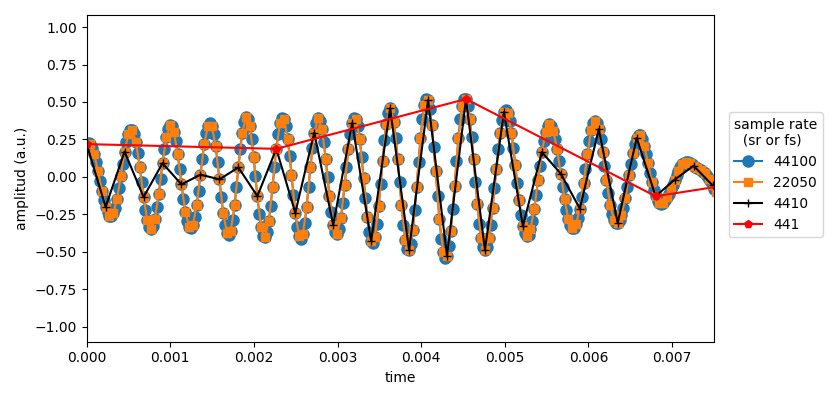
\includegraphics[width=\linewidth]{Images/fs.png}
    \caption{Sampling rate or sampling frequency of a continuous noisy signal. Note how with at lower sampling rates the sampled signal does not correctly reproduces the original signal. In order to do not to loss the function behavior, the sampling rate must satisfy the sampling theorem: the signal has to be sampled with at least twice the frequency of the original signal.}
    \label{fig:sampling_rate}
\end{figure}


\subsubsection{Envelope}

The sound envelope describes how the amplitude of the sound changes over time. It is not an instantaneous measurement, it is a curve such that it covers the audio signal and is calculated with its extreme points or percentiles. In this work, the envelope of a function $x(t)$ will be denote as $e(t)$. 


\subsection{Spectral Analysis}

In the previous section sound was studied and defined as a sequence of numbers that usually depends of the time, this mathematical representation allows the visualization and modification of audio. This approach to study  is called time domain analysis and exploring the audio by its amplitude, although sometimes is good enough in many other cases it is not enough. \\

A more powerful tool is the spectral analysis, where the signal of interest is studied in the frequency domain. This analysis aims to characterize the frequency content of a signal by decomposing it into an orthogonal basis of periodic functions: the object is to find the coefficients of the expansion that gives the amplitude (or weight) of its corresponding frequency.\\

Let us define some terms and spectral characteristic that this work used.


\subsubsection{Fourier Series (FS)}

The goal of the spectral analysis is to decompose the signal into its frequency, find the best basis and expansion coefficients for the signal. But, what is the best approximation?

The answer to this question will depend of the nature of the phenomena, the best basis is the function that best emulates the behavior of the phenomena. Therefore, it is natural to think that for audio signals, and many other digital signals, the best basis functions are trigonometric functions, which are periodic and easily differentiable.\\

Any function can be approximate by a linear combination of a basis function, in particular this functions can be a Laurent polynomial
\begin{equation*}
    f(x) \approx \sum_{n=-N}^N c_n q^n(x)
\end{equation*}
which are polynomials with positive and negative power terms. Although polynomials are solid basis, not all problems are well defined with them.\\

Other important basis functions are the trigonometric polynomials, these polynomials of degree $N$, $p:\mathbb{C}\to\mathbb{C}$, has the following form
\begin{equation*}
    p(x) = \sum_{n=-N}^N c_n e_n(x)
\end{equation*}
where $c_n \in \mathbb{C}$ are some coefficients to be calculated and $e_n(x)=e^{2\pi i n x}$ is the basis function with $n\in\mathbb{Z}$. Note that the expansion basis is the exponential function which is related to the trigonometric function by the Euler's formula
\begin{equation*}
    \int_0^1 e^{2\pi i n x} dx = \cos (2\pi  n x) + i \sin (2\pi n x)
\end{equation*}
This base is a good election since it is orthonormal
\begin{equation*}
    e^{2\pi i n x} \; \cdot \; e^{2\pi i m x} = \delta_{m,n}
\end{equation*}
which implies
\begin{equation*}
    \int_0^1 p(x) \overline{e_n(x)} dx = c_n
\end{equation*}
It is very useful to calculating the coefficients, but $f$ must be integrable if its domain is the complex set and a square-integrable function\footnote{a function is called square-integrable function if $\int_{-\infty}^\infty |f(x)|^2 dx < \infty$} if its domain is the real numbers. Then, the $nth$ Fourier Coefficient of $f$ is defined as
\begin{equation*}
    \hat{f}(n) = \int_0^1 p(x) \overline{e_n(x)} dx 
\end{equation*}
In the same way, the $Nth$ Fourier polynomial $f_N$ of $f$ is
\begin{equation*}
    f_N(x) =  \sum_{n=-N}^N \hat{f}(n) e_n(x) 
\end{equation*}
In other words, $f_N(x)$ is the the trigonometric polynomial of degree $N$ whose coefficients are the Fourier coefficients $\hat{f}(n)$.\\

Using this polynomial, a "good approximation" means that $f_N$ is an approximate function of $f$ when $N\to \infty$, $\lim_{N\to \infty} f_N = f$.
\begin{equation}\label{eq:Fourier_serie}
    f(x) = \lim_{N\to \infty} f_N(x) = \sum_{n=-\infty}^\infty \hat{f}(n) e_n(x) = \sum_{n\in \mathbb{Z}} \hat{f}(n) e_n(x) 
\end{equation}
although the equal symbol is present, it is an approximation of the function because the calculation of the series produces truncation errors. Using the Euler's relations
\begin{equation*}
    f(x) = \sum_{k=0}^\infty A_k \cos \left( \frac{2\pi k}{T}x \right) + \sum_{n=0}^\infty  B_k \sin \left(\frac{2\pi k}{T}x \right)
\end{equation*}
where $T$ is the common period of the function $f(t)$ and its the fundamental frequency is $f_1=1/T$. \cite{fourier_signal, fourier_math}

\subsubsection{Fourier Transform (FT)}

This transformations is a generalization of the Fourier series (FS), it is the continuous analog; instead of calculating the discrete values of the Fourier coefficients $\hat{f}(n)$ with $n\in \mathbb{Z}$, the transformation takes continuous values $\hat{f}(x)$ for $x\in \mathbb{C}$. This transformation is defined as 
\begin{equation}\label{eq:fouerir_transform}
    \hat{f}(\omega) = \int_{-\infty}^{\infty} f(x) e^{-2\pi i \omega x} dx, \qquad f(x) = \int_{-\infty}^{\infty} \hat{f}(\omega) e^{2\pi i \omega x} d\omega
\end{equation}
the right-hand side is the inverse transformation, this transformation recovers $f$ from its Fourier coefficients $\hat{f}(\omega)$ with $\omega\in \mathbb{C}$.\\

The Fourier transformation is a linear transformation $\mathcal{F}: \mathbb{C} \to \mathbb{C}$of the function $f$, it will be denoted as $F(\omega)=\mathcal{F} \{ f(x)\} = \hat{f} (\omega)$.


\subsubsection{Discrete Fourier Transform (DFT) }

The discrete Fourier Transform (FT) transform a sequence of $N$ elements,$\{x_K\}:=x_0, x_1,\dots, x_{N-1}$, into another sequence of complex numbers, $\{X_K\}:=X_0, X_1,\dots, X_{N-1}$, which is defined as
\begin{align}\label{eq:FT}
    &X_k  = \sum_{n=0}^{N-1} x_n e^{-\frac{2\pi i}{N}kn} \\ 
    X_k &= \sum_{n=0}^{N-1} x_n \; \left[\cos \left( \frac{2\pi}{N}kn\right) -i \;  \sin \left(\frac{2\pi}{N}kn \right)\right]
\end{align}


\subsubsection{Fast Fourier Transform (FFT)}

A fast and efficient algorithm to compute the discrete Fourier transform (DFT) or its inverse (IDFT). This algorithm rapidly computes such transformations by factorizing the DFT matrix into a product of sparse (mostly zero) factors. \cite{signal_book_modern}
\begin{equation}\label{FFT}
    X_K = \sum_{n=0}^{N-1} x_n e^{-2\pi ikn/n}, \qquad k=0,1,\dots, N-1
\end{equation}
where $x_k\in \mathbb{C}$ and $e^{-2\pi i/n}$ a primitive root.

\subsubsection{Short-Time Fourier transform (STFT)}

\begin{equation}\label{STFT}
    \textbf{STFT}\{x(t)\}(\tau, \omega) = \int_{-\infty}^\infty x(t) w(t-\tau )e^{-i\omega t} dt = \mathcal{F} \{ x(t)w(t-\tau)\}
\end{equation}
where $w(t)$ is the window function (commonly Gaussian, Hann, or Hamming windows)


\begin{equation}\label{STFT}
    \textbf{DSTFT}\{x(t)\}(n, \omega) = X(n,\omega)= \sum_{n=-\infty}^\infty x[n] w [n-m]e^{-i\omega n} 
\end{equation}

\subsubsection{Convolution Theorem}

This theorem states that under suitable conditions the Fourier transform of a convolution of two functions (or signals) is the pointwise product of their Fourier transforms.

\begin{gather}\label{convolution_theorem}
    \mathcal{F} \{ f * g\} = \mathcal{F} \{ f \} \mathcal{F} \{  g\} = f*g
\end{gather}


\subsubsection{Spectrograms}

A spectrogam is a graphic representation of a recorded
sound (like a bird song) that includes information on
both frequency and loudness, usually by plotting frequency against time and indicating intensity by shading or colors. It usually also called power spectrum and denoted by $S_{xx}(x(t))$ where $x(t)$ is the time series signal. Mathematically speaking, spectrograms are defined as the energy spectral density as follows
\begin{equation}\label{spectro_STFT}
    S_{xx} = spectrogram\{x(t)\} (\tau,\omega) = |X(\tau, \omega)|^2
\end{equation}
This visualizations are usually heatmaps, i.e., as an image with the intensity shown by varying the colour or brightness. When are plotted in three-dinemnsions are called waterfall plots.

\subsubsection{Power Spectral Density (PSD)}

It is a power spectrum (spectrogram) of a signal which describes the power present in the signal as a function of frequency, per unit frequency. Power spectral density is commonly expressed in watts per hertz (W/Hz) while power spectrum in dbS or dBFS.

\subsubsection{Mel Spectrogram (MFCC)}

The mel-spectrogram is often log-scaled before, it remaps the values PSD in hertz to the mel scale. MFCC is a very compressible representation, often using just 20 or 13 coefficients instead of 32-64 bands in Mel spectrogram. The MFCC is a bit more decorrelarated than other spectrograms representations which is beneficial for some application like Gaussian Mixture Models.


\subsubsection{Fundamental Frequency}

It is the lowest frequency produced by the oscillations of an object. The fundamental frequency is also called the first harmonic of the instrument or pitch.\\

Although there are many ways to compute it, the most used algorithm to the pithc extraction is the YIN (or the probabilistic version PYIN) algorithm. This algorithm compute an estimation of the fundamental frequency ($F_0$) of speech or musical by following the next steps:

\begin{enumerate}
    \item[\textbf{Step 1:}] The autocorrelation method, uses the autocorrelation function (ACF).
    \item[\textbf{Step 2:}] Difference function.
    \item[\textbf{Step 3:}] Cumulative mean normalized difference function.
    \item[\textbf{Step 4:}] Absolute threshold.
    \item[\textbf{Step 5:}] Parabolic interpolation
    \item[\textbf{Step 6:}] Best local estimate
\end{enumerate}

This algorithm is already implemented and tested by librosa \cite{yin, librosa}.

\subsubsection{Harmonics}

A harmonic is a wave or signal whose frequency is an integral (whole number) multiple of the fundamental frequency of the same reference signal or wave. The presence of harmonics in a signal depends of the nature of the signal. Birds and human vocalization usually have harmonics.

%\subsubsection{RMS Frequency}
\subsubsection{Mid Spacial Frequency ($f_{msf}$)}

The mid spacial frequency is defined as the average of the frequencies presented in the sound pondered by the sound energy.

\begin{equation}
    f_{msf} = \frac{1}{E} \sum_{i=1}^N f_i 
\end{equation}

%\subsubsection{Spectral Centroid}


\subsection{Acoustic Indexes}

This indexes are used to characterize the signal properties, both in spectral and time domain
\subsubsection{Power Spectral Entropy (SE)}

\begin{equation}\label{eq_spectral_entropy}
  PSE (F) = -\frac{1}{\log N_n}   
\end{equation}



\subsubsection{Spectral Content Index (SCI)}

Index with information about the spectral content of a signal. Simple signals has a SCI close to 1 while for complex signals the index value increase.

\begin{gather}\label{eq_SCI}
    SCI = \frac{f_{msf}}{FF}
\end{gather}



% \subsubsection{Spectral Entropy (SE)}
% \subsubsection{Acoustic Complexity Index (ACI)}

\subsubsection{Acoustic Dissimilarity}

Indexes used to compute how similar are two set of Fourier coefficients. Let $x$ and $y$ two $N$ point Mel mean spectral of interest, $x,y\in \mathbb{R}^N$, then the acoustic dissimilarity can be calculated with any of the following indexes


\begin{itemize}
    \item Correlation-based dissimilarity
    
    \begin{equation}\label{correlation_eq}
        correlation = \sqrt{1-\frac{||x\cdot y||_1}{||x||_2 \;||y||_2}}
    \end{equation}
    
    \item Symmetric Kullback–Leibler divergence
    \begin{equation}\label{SKL_eq}
        KL = \frac{1}{2} \sum_i^N \left(x_i \log_2\left|\frac{x_i}{y_i}\right| + y_i \log_2\left|\frac{y_i}{x_i}\right|  \right)
    \end{equation}
    
    
    \item The integral of pointwise difference
    \begin{equation}\label{SKL_eq}
        D_f = \frac{1}{2} \sum_i^N |x_i-y_i| %|||x-| ||_1
    \end{equation}
    
    Acoustic indexes definition taken from \cite{dissimilarity_acoustic_indices}
\end{itemize}

This indexes are from 0 to 1, where 1 represents great similar between Fourier coefficients.


\section{Dynamical Systems}\label{sec_non_linear_dynamics}

In general terms a dynamical system is any system, natural or man-made, that changes over time: the water cycle, the electron moving around proton, or even climate change... there are an endless numbers of examples and the birdsongs is one of them.\\

Formally speaking, a dynamical system is a system such that a set of variables uniquely define its state and with an associated \textbf{rule} to describe its behavior over time. \textbf{Differential equations} are used to study dynamical systems with physical modeling involved to describe the system at an instant in terms of some variables set called \textbf{state space}, or state variables, a n-dimensional point $x\in \mathbb{R}^n$ that depends of the complexity of the system. Depending on the nature of system, it can be described in discrete time steps or on a continuous timeline, but in either cases the state will be defined by a \textit{difference equation} (or an iterative map) 
\begin{gather}\label{difference_equation}
    x_{t} = f(x_{t-1},t)  \qquad \text{(discrete)}\nonumber\\
    \frac{dx}{dt}= f(x,t) \qquad \text{(continuous)}
\end{gather}
where $f$ is a function defined by system evolution time rule. If the time of the system is continuous and deterministic, the system is defined by a \textbf{flow}, also called flow map and define as $x(t)=\phi_t(x(0))$. Dynamical system are either \textbf{deterministic}, given an initial point the final state is defined by a unique state, or \textbf{stochastic}, or random if there is a probability distribution. In any case, a dynamical system is described mathematically by an \textit{initial value problem (IVP)} which implies a notion of time, in fact a state at one time will evolves to another possible state or collection of states, as a single quantity used to order the states chronologically. \cite{scholarpedia}


\section{Bifurcation Theory}

A bifurcation is the division of something into two parts. The same idea is used by bifurcation theory, which studies the mathematical changes in the topological or qualitative structure of a family of curves and the solutions of a family of differential equations, which studies how the sates of system bifurcate. In particular, for dynamic systems a bifurcation occurs when a small change in values of the system's parameters causes a sudden qualitative change in its behavior; for examples the dynamic system starts and ends to oscillating at certain critical points. \cite{bifurcation} \\

A formal definition starts from considering a set of ordinary differential equations, $\dot{x} = f(x, \lambda)$, which depends of a n-dimensional variable $x\in\mathbb{R}^n$, $p$ parameters $\lambda\in\mathbb{R}^p$, and a smooth time rule function $f : \mathbb{R}^{n+p} \to \mathbb{R}^n$. Then, a bifurcation occurs when $\lambda$ takes a close value $\lambda_1$ such that the the number or stability of equilibria points or periodic orbits of $f$ changes significantly. \\

An interesting way to think of bifurcations can be as a failure in the stability of the system within a family. To classify bifurcations we study their stability with the Kupka-Smale theorem which lists three generic properties of vector fields:

\begin{itemize}
    \item Hyperbolic equilibrium points.
    \item Hyperbolic periodic orbits.
    \item Transversal intersections of stable and unstable manifolds of equilibrium points and periodic orbits.
\end{itemize}

In addition, the term \textbf{codimension} is used to describe the number of equality conditions that characterize the bifurcation, i.e. the minimum number of parameters if families in which the bifurcation take place. \\

A single failure in the Kupka-Smale properties yield to divide codimension one bifurcations in the following bifurcations types:

\begin{itemize}
    \item Equilibria
    \begin{itemize}
    \item Saddle - Node
    \item Andronov-Hopf 
    \end{itemize}
    
    \item Periodic Orbits
    \begin{itemize}
    \item Fold Limit Cycle
    \item Flip Bifurcation (aka Period Doubling)
    \item Neimark-Sacker Bifurcation (aka Torus)
    \end{itemize}
    
    
    \item Global Bifurcations
    \begin{itemize}
    \item Homoclinic Bifurcation of equilibria
    \item  Homoclinic tangencies of stable and unstable manifolds of periodic orbits
    \item Heteroclinic Bifurcation of equilibria and periodic orbits
    \end{itemize}
    
\end{itemize}



In this work, the dynamical system of study (the avian vocal organ) will present interesting behaviors with Saddle-Node, Hopf, and limit cycle bifurcations. The global bifurcation involving all these bifurcations is the 
Bogdanov–Takens bifurcation that will be explained in section \ref{Bogdanov_Takens_Bifurcation}.\\

Any study of bifurcation begins by examining the \textbf{equilibrium points} (also called equilibrium or \textit{fixed points}) of the dynamical system. These points are generated by the system of ordinary differential equations (ODEs) and are time-invariant solution. Mathematically speaking, the ODE $x'=f(x)$ has an equilibrium solution (or a steady state) $x(t)=x_e$ if this point is a root of the ODE function $f(x_e)=0$. Although the process is fairly straightforward, it is not always easy to solve the equation $f(x)=0$ and it is only  possible in some special cases. \cite{bifurcation}

\subsection{Types of Equilibria}

To equilibria of the bifurcations are studied by calculating the egienvalues and eigenvectors of the time function rule $f$ with the Jacobian matrix associated to the dynamical system, defined as

\begin{equation}\label{Jacobian}
    J(x) :=\frac{\partial f_i}{\partial x_j} = \begin{pmatrix} \nabla^T f_1 \\ \vdots \\ \nabla^T f_n
    \end{pmatrix} =\begin{pmatrix} \frac{\partial f_1}{\partial x_1} & \cdots & \frac{\partial f_1}{\partial x_n}\\
    \vdots & & \vdots \\
    \frac{\partial f_n}{\partial x_1} & \cdots & \frac{\partial f_n}{\partial x_n}\end{pmatrix}
\end{equation}

where $\nabla^T f_i$ is the transpose of the gradient of the $i$ component. By evaluating the Jacobian matrix at the equilibrium point, all derivatives, and then calculating its eigenvalues it is possible to determine the linear stability properties of the equilibrium point. Then, the Jacobian has same number of egienvalues as the dimension of the variables vector; if all egienvalues have negative parts the equilibrium is called \textbf{asymptotically stable}, if at least one eigenvalue has positive real part is called \textbf{unstable}, and it is said to be \textbf{hyperbolic} if all the eigenvalues have non-zero real parts, or \textbf{non hyperbolic} if at least one eigenvalue is null or has a zero real part. \\

While hyperbolic equilibria are robust, small perturbations does not causes qualitative changes to the phase space near to the equilibria point, non hyperbolic equilibria are not, small perturbations can cause a local bifurcation that change stability, vanish or split into many equilibria points, and are called \textit{saddle-node equilibrium}.\\

Let us consider some examples of spaces for usual bifurcations.


% \begin{figure}[H]
% \begin{tabular}{cc}
%     \begin{minipage}{0.6\textwidth} \begin{subfigure}{\linewidth}
%     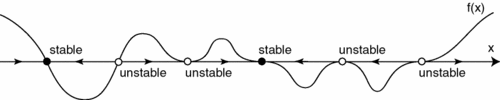
\includegraphics[width=0.9\linewidth]{Images/1d.png}
%     \caption{Diagram bifurcation for a one-dimensional dynamical system $x'f(x)$, the equilibrium points are the roots of $f$. } \label{subfig:1d}\end{subfigure}
%     \vspace*{0.6cm} 
%     \begin{subfigure}{\linewidth}
%     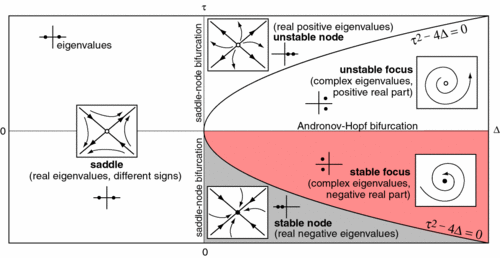
\includegraphics[width=0.9\linewidth]{Images/2d.png}
%     \caption{Two-dimensional dynamical system types of equilibrium points that depends of the Jacobian trace ($text{tr}$) and determinant ($\Delta$). The red and gray shadow regions corresponds to stable equilibrium points.} \label{subfig:2d}\end{subfigure}
%     \end{minipage}
%     \begin{minipage}{0.4\textwidth} 
%     \begin{subfigure}{\linewidth}
%     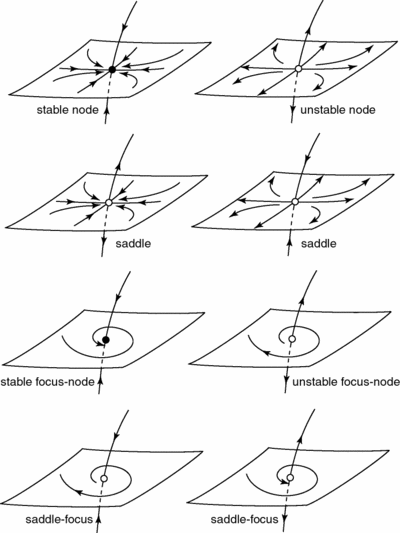
\includegraphics[width=0.9\linewidth]{Images/3d.png}
%     \caption{Equilibrium points examples for a three-dimensional dynamical system.} \label{subfig:3d}\end{subfigure}
% \end{minipage}
% \end{tabular}
% \caption{Dimensional spaces of equilibria \label{fig:spaces}}
% \end{figure}

\subsubsection{One-Dimensional Space}

Let us consider a scalar dynamical system defined by a differentiable function $f\in C^1$, $x' = f(x)$, with $x\in\mathbb{R}$. The equilibria points are the root of the function $f$, as shows Figure \ref{fig:1d} where the first two points are hyperbolic and the other non-hyperbolic\footnote{because the y-component of the slope is zero, the eigenvalue of the Jacobian matrix}. If the Jacobian $J=f'(x)$ at the root is negative it is a stable point $f'(x)<0$, while if it is positive at the point $f'(x)>0$ it is an unstable point.

\begin{figure}[H]
    \centering
    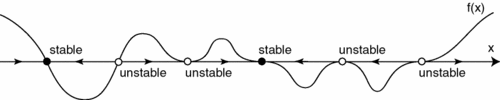
\includegraphics[scale=0.85]{Images/1d.png}
    \caption{Diagram bifurcation for a one-dimensional dynamical system $x'f(x)$, the equilibrium points are the roots of $f$.}
    \label{fig:1d}
\end{figure}

\subsubsection{Two-Dimensional Space}

A more interesting case is two-dimensional bifurcations. Let us consider a two-dimensional dynamical system defined as a set of ordinary differential equations
\begin{gather*}
\begin{matrix}
x_1'=f_1(x_1,x_2)\\
x_2'=f_2(x_1,x_2)
\end{matrix}, \qquad J(x_1,x_2) = \begin{pmatrix} \frac{\partial f_1}{\partial x_1} & \frac{\partial f_1}{\partial x_2}\\\frac{\partial f_2}{\partial x_1} & \frac{\partial f_2}{\partial x_2}\end{pmatrix}
\end{gather*}

Since the space is two-dimensional the Jacobian matrix has two eigenvalues that are either both real or complex-conjugate, defined by the trace and determinant of the Jacobian defined as follows
\begin{gather*}
    \tau = \text{tr}J = \frac{\partial f_1}{\partial x_1} +\frac{\partial f_2}{\partial x_2}\\
    \delta = \text{det} J = \frac{\partial f_1}{\partial x_1} \frac{\partial f_2}{\partial x_2}- \frac{\partial f_2}{\partial x_1} \frac{\partial f_1}{\partial x_2}
\end{gather*}

\begin{figure}[H]
    \centering
    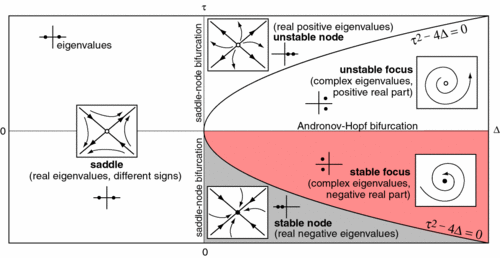
\includegraphics[width=\linewidth]{Images/2d.png}
    \caption{Two-dimensional dynamical system types of equilibrium points that depends of the Jacobian trace ($text{tr}$) and determinant ($\Delta$). The red and gray shadow regions corresponds to stable equilibrium points.}
    \label{fig:2d}
\end{figure}

Both hyperbolic and non-hyperbolic equilibrium points are present in this dynamical system: nono-hyperbolic equilibria are located on the half-axis $\tau =0$, $\Delta>0$, and on the axis $\Delta=0$ arising at the Andronov-Hopf and at Saddle-Node bifurcation, respectively; while a hyperbolic equilibrium can be: 

\begin{itemize}
    \item \textbf{Saddle}, both eigenvalues are real and of opposite signs then the point is unstable.
    \item \textbf{Node}, both eigenvalues are real and of positive signs. The point is stable is the eigenvalues are negative and unstable when they are positive.
    
    \item \textbf{Spiral point (or focus)}, the eigenvalues are complex-conjugate. It is stable if the eigenvalues have negative part and unstable when they have positive part.
\end{itemize}

Figure \ref{fig:2d} summarize the types of equilibrium for a two-dimensional dynamical system.

\subsubsection{Three-Dimensional Space}

In this case the Jacobian matrix has three eigenvalues, one of them must be real and the other two can be either both real or complex-conjugate. Figure \ref{fig:3d} shows the interesting possible cases for this dynamical system that are defined by the type and sign of the eigenvalues. Similar to two-dimensional dynamical system, a hyperbolic equilibrium can be: \\

\begin{itemize}
    \item \textbf{Node}, all eigenvalues are real and have the same sign. If the eigenvalues are positive (negative) the point is unstable (stable).
    \item \textbf{Focus-Node}, all eigenvalues have real parts of the same same where one eigenvalue is real and the others are a complex-conjugate pair. It is a stable (unstable) point when the sign is negative (positive).
    \item \textbf{Saddle}, all eigenvalues are real and at least one of them is positive and at least one is negative. They are always unstable points.
    \item \textbf{Saddle-Focus}, one real eigenvalue with the sign opposite to the sign of the real part of a pair of complex-conjugate eigenvalues. It is always an unstable point.
\end{itemize}


If time is reversed, changing $t\to -t$, the node and focus-nodes change their stability, while in contrast saddle and saddle-focus remain unstable.


\subsubsection{Non-Hyperbolic Equilibria}

These are not the only types of non-hyperbolic equilibria, those points having at least one eigenvalue with zero real part, three other examples in $\mathbb{R}^2$ are displayed in the Figure \ref{fig:4d}.


\begin{itemize}
    \item \textbf{Center equilibrium}, a pair of purely imaginary eigenvalues. These points in linear system have families of concentric periodic orbits. 
    
    \item \textbf{saddle-node equilibrium}, one zero eigenvalue in a nonlinear system undergoing a saddle-node bifurcation, the equilibria is always unstable. Here a saddle and node approach each other and merge into a single equilibrium point and then disappear.
    
    \item \textbf{Bogdanov-Takens equilibrium}, two zero eigenvalues of a nonlinear system that usually undergoes a Bogdanov-Takens bifurcation. As well as saddle node it is an unstable equilibrium.
\end{itemize}


\begin{minipage}{0.45\linewidth}
\begin{figure}[H]
    \centering
    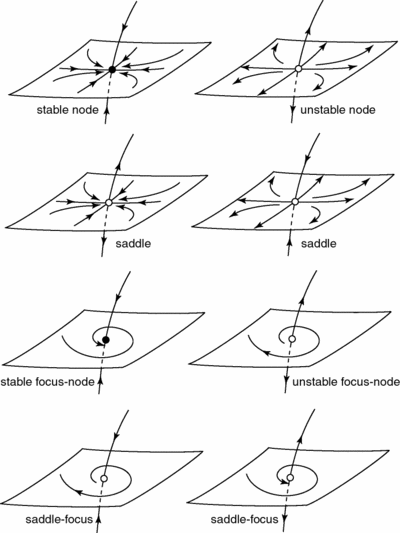
\includegraphics[width=\linewidth]{Images/3d.png}
    \caption{Equilibrium points examples for a three-dimensional dynamical system.}
    \label{fig:3d}
\end{figure}
\end{minipage}\hspace{10pt}
\begin{minipage}{0.45\linewidth}
\begin{figure}[H]
    \centering
    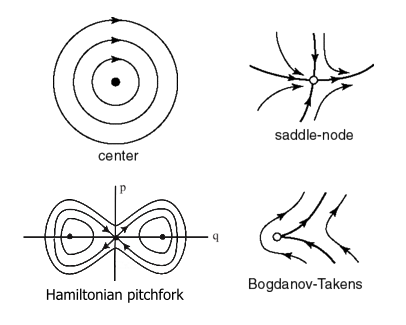
\includegraphics[width=1.1\linewidth]{Images/4d.png}
    \caption{Non-hyperbolic equilibrium points in $\mathbb{R}^2$. The center and Bogdanov-Takens bifurcation diagrams correspond to Hamiltonian equations, $x''=-\omega^2 x$ and $x''=Kx^2$, respectively.}
    \label{fig:4d}
\end{figure}
\end{minipage}



\subsection{Andronov-Hopf}

This bifurcation consist of a change in stability by a pair of pure imaginary eigenvalues that generate a limit cycle solution\footnote{a special type of solution for a dynamical system that repeats itself in time}. There are two possible types of limit cycles: \textbf{supercritical} and \textbf{subcritical}, stable and unstable respectively, Figure \ref{fig:hopf_types}.


\begin{figure}[H]
     \centering
     \begin{subfigure}[b]{0.7\textwidth}
         \centering
         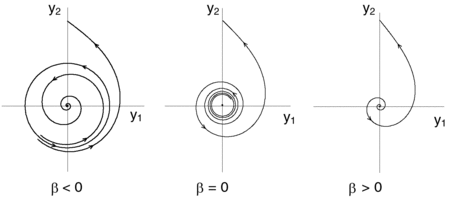
\includegraphics[width=\textwidth]{Images/SubHopf.png}
         \caption{Supercritical bifurcation}
         \label{fig:sub_hopf}
     \end{subfigure}
     \hfill
     \begin{subfigure}[b]{0.7\textwidth}
         \centering
         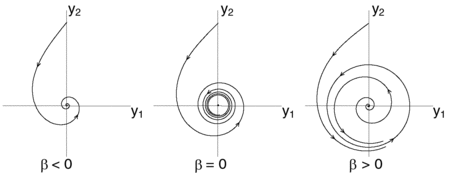
\includegraphics[width=\textwidth]{Images/SuperHopf.png}
         \caption{Supercritical bifurcation}
         \label{fig:sup-hopf}
     \end{subfigure}
     \hfill
        \caption{Hopf possible types of bifurcations.}
        \label{fig:hopf_types}
\end{figure}


\subsection{Saddle-Node}

This bifurcation occurs when the critical equilibrium has one zero eigenvalue. It is also called fold or limit point bifurcation and consists in the creation, collision, and destruction of two critical points, as shows the Figure \ref{fig:saddle-node}.
.
\begin{figure}[H]
    \centering
    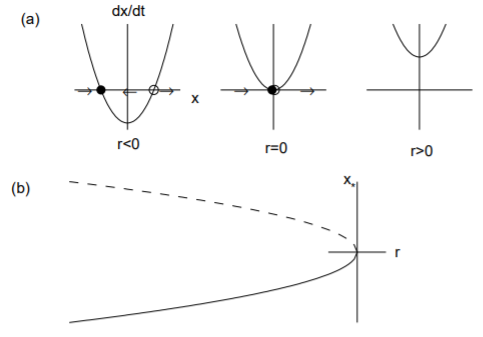
\includegraphics[scale=0.75]{Images/saddle-node.png}
    \caption{One dimensional saddle-node bifurcation $x'=r+x^2$. (a) Phase space, $x'$ vs $x$. (b) bifurcation diagram }
    \label{fig:saddle-node}
\end{figure}

\subsection{Limit Cycle}



\begin{minipage}{0.45\linewidth}
When the solution of the dynamical system is a stable periodic orbit, it is called a limit cycle or oscillator. This bifurcation is fascinating as they fill generate oscillating dynamical systems. \\

The stability of a periodic orbit is calculated using Poincare maps. If all eigenvalues have a modulus value less than unit the corresponding bifurcation is asymptotically stable, but if instead its modulus is greater than unit then the bifurcation is unstable.

\end{minipage}\hfill
\begin{minipage}{0.45\linewidth}
\begin{figure}[H]
    \centering
    \animategraphics[loop,width=\linewidth]{17}{Images/cycle/cycle}{1}{20}
    \caption{Periodic orbit shown in phase space, simple harmonic motion}
    \label{fig:air_motion}
\end{figure}
\end{minipage}



\subsection{Bogdanov–Takens (BT) Bifurcation}\label{Bogdanov_Takens_Bifurcation}

It consists of an equilibrium point that bifurcates into a two parameter family solutions of the ODE \eqref{eq:Bogdanov_Takens_Bifurcation}. The equilibrium point has two degenerated zero eigenvalues, of multiplicity two. The ordinary differential equation system is
\begin{gather}\label{eq:Bogdanov_Takens_Bifurcation}
    x_1' = x_2\nonumber\\
    x_2 ' = \alpha + \beta x_1 + x_1^2-x_1x_2 \\
    (\text{or }x_2 '=-\alpha -\beta x_1 + x_1^2-x_2^3-x_1x_2-x_1^2x_2) \nonumber
\end{gather}


\begin{figure}[H]
    \centering
    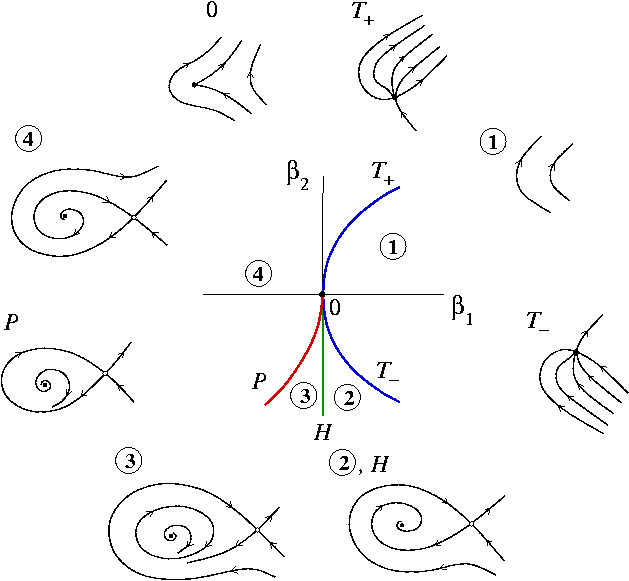
\includegraphics[scale=0.75]{Images/BogdanovTakens.png}
    \caption{Bogdanov-Takens bifurcation, possible solutions of parameters families.}
    \label{fig:takens}
\end{figure}

Close parameters values generate two equilibrium points, a saddle and nonsaddle, which collide and vanish via a saddle-node bifurcation. An Andronov-Hopf bifurcation is generated by the nonsaddle equilibrium that produces a limit cycle. This cycle degenerates into an homoclinic orbit to the saddle and disappears via a saddle homoclinic bifurcation. \cite{bifurcations_book, bifurcation}


\section{Numerical Optimization}

Throughout the entire history of the universe  nature and livings beings have been evolving to survive, to continue living as mush as possible, leading them to reach the current evolution where we have develop wireless communications, for faster and easier interactions, flying machines, to travel huge distances in a few hours, and even bionic eyes, to see the quantum and cosmic world, but all these inventions have the same idea behind: \textit{how to improve a something}: how to get betters results from a problem by understanding its nature and what it depends o?n. But, what does better results mean?\\

To define and quantify the phrase "better results", the theory of mathematical optimization emerges and creates a robust mathematical tool, with many concepts, algorithms, and theorems, to solve any kind of optimization problem, or any problem that can be written as one. \\

This chapter is an introduction to numerical optimization, defining and discussing the necessary concepts and theory used in this work. \cite{numerical_opt}

\subsection{Introduction}

First, any optimization problem must have a defined \textbf{objective function}: a quantitative score that measures the performance variable of the system of interest, usually a profit, time, energy, or any physical variable of the system; it depends on system characteristic which are called \textbf{variables}. The goal of optimization is to find \textbf{optimal} variables that minimize (or maximize) the objective function subject to some \textit{constraints} that the system must satisfy.\\

In many cases the domain of the problem variables are constraint to some region, the variables limits are well determined and it is possible to define the \textbf{feasible domain} on the problem. The constraints and objective function can be linear, quadratic, or nonlinear functions, and may depend of some known values \textbf{parameters} which characterize the system under study.\\


In optimization, \textbf{modeling} is the process of identify the objective function, constraints and system variables. Any optimization problem has behind it a modeling process, the most important step, where the limits and scopes of the model are determined. Once the problem has been modeled, the next step is to apply an optimization algorithm to find the \textbf{optimal variables} and check if they are indeed the solution of the problem by means of some mathematical expressions called \textbf{optimal conditions}. At this point the problem has an optimal set of variables but sometimes it is not enough. To improve the modeling process a \textbf{sensitive analyze} can be used, which reveals how sensitive is the model to changing input data or parameters  values. 

\begin{figure}[H]
    \centering
    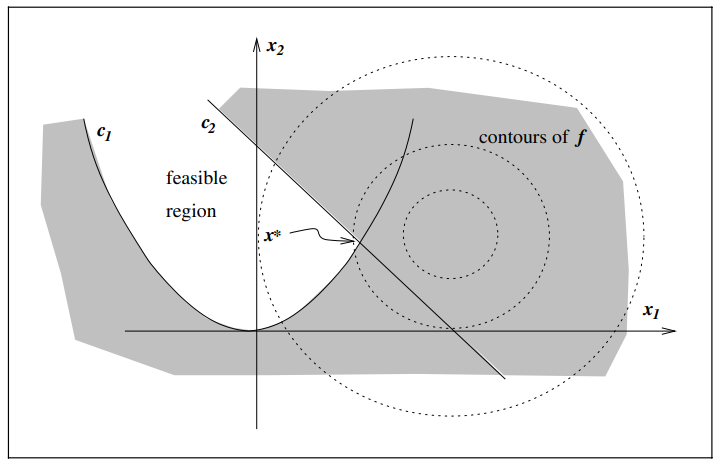
\includegraphics[scale=0.65]{Images/problem_opt.png}
    \caption{Geometrical representation of an optimization problem. \cite{numerical_opt}}
    \label{fig:opt_problem}
\end{figure}


Therefore, the optimization objective can be summarized as the minimization or maximization of a function whose variables must satisfy some constraints. Although the objective function have to be scalar, many problems functions can be written as vector functions and then the problem can though of as minimizing (or maximizing) a vector norm. Depending of the nature an behavior of the objective function and constraints, whether they are linear, quadratic, non smooth, or nonlinear functions, the optimization algorithm is chosen. With these properties, optimization theory classifies and studies the problems, in addition, the presence (or not) of constraints is also important and allows another classification to the problems,  \textit{constraint or unconstrained optimization}.

\subsubsection{Mathematical Formulation}

Using mathematical notation, an optimization problem can be written as follows
\begin{equation}\label{math_opt}
\begin{aligned}
\underset{ x \in \mathbb{R}^n}{\text{min}} &\quad   f(x)\\
    \text { subject to }  & \quad  \;   c_i(x)=0, \quad i \in \mathcal{E} \text {, }\\
    & \quad  \; c_i(x) \geq 0, \quad i \in \mathcal{I}
\end{aligned}
\end{equation}

here $x$ is the vector of variables (also called unknowns or parameters), $f:\mathbb{R}^n\to\mathbb{R}$ the scalar objective function, $c_i$ scalar constraints  functions that that must satisfies the vector variables where $\mathcal{E}$ and $\mathcal{I}$ are the indices for equality and inequality constraints, respectively. 

\subsubsection{Convexity}

An important property of a function or set in optimization is the \textit{convexity}. In fact, a wide variety of problems posses this property that make them easier to solve in theory and in practice, they are studied and solved with the theory of \textbf{convex optimization}.\\

A set $S$ is called convex if the straight line segment connecting any two points of $S$ lies entirely inside $S$, formally speaking for any two points $x,y\in S$, then $\tau x +(1-\tau)y \in S$ for all $\tau in [0,1]$. Similarly, a function $f$ is convex if its domain $S$ is a convex set and if for any two point of $x,y \in S$, the following property is satisfied

\begin{equation}\label{convecity}
        f(\tau x+(1-\tau) ) \leq\tau f(x) + (1-\tau)f(y), \quad \text{for all } \tau \in [0,1] 
\end{equation}

This property is important because if the objective function and its domain satisfy it, then any local solution of the problem is in fact a global solution. For the special case where everything is convex, the objective function and constraints, the term \textit{convex programming} is used.


\subsubsection{Optimal Solution} % Local and Global

Depending of the nature and properties of the function, the problem would have a \textbf{global minimizer (maximizer)} or \textbf{local minimizer (maximizer)}, the optimal solution. The ideal case is to find a global optimizer of the objective function $f$. It is define as point $x^*$ such that 
\begin{gather*}
    f(x^*) \leq f(x)  \forall x \in D \quad (\text{global minimizer})\\
    f(x^*) \geq f(x) \forall x \in D \quad(\text{global maximizer})
\end{gather*}

where $D$ is the problem domain of interest which can be the a real set $\mathbb{R}$. Sometimes it is difficult to find the global optimizer since our knowledge of the objective function is only local. Usually a local optimizer is sufficient for some problems and the most optimization algorithms are able to find them. A point $x^*$ is called \textbf{local optimizer} (minimizer or maximizer) if there is some neighborhood $N$ such that
\begin{gather*}
    f(x^*) \leq f(x), \; \forall x \in N\quad (\text{local minimizer})\\
    f(x^*) \geq f(x), \; \forall x \in N \quad(\text{local maximizer})
\end{gather*}

where this neighborhood is an open set that contains $x^*$. When the point satisfied any of this inequalities is called \textit{weak local optimizer}. Similarly, a \textbf{stric local optimizer}, the best optimal of the neighborhood, is a point such that

\begin{gather*}
    f(x^*)< f(x) \forall \in N, \; \text{with } x \neq x^* \quad \text{(\textbf{stric local minimizer})}\\
    f(x^*)> f(x) \forall \in N, \; \text{with } x \neq x^* \quad \text{(\textbf{stric local maximizer})}
\end{gather*}

\begin{minipage}{0.45\linewidth}
Therefore, to find an optimal point a basic but expensive algorithm can be scan the whole feasible region, dividing this region into a grid of points and computing the objective function at each point. This technique for solving the problem is a \textbf{brute-force search}, it is easy to implement and always finds a solution if one exist, but the implementation is very expensive as it depends of the number of candidates.
\end{minipage}\hfill
\begin{minipage}{0.45\linewidth}
\begin{figure}[H]
    \centering
    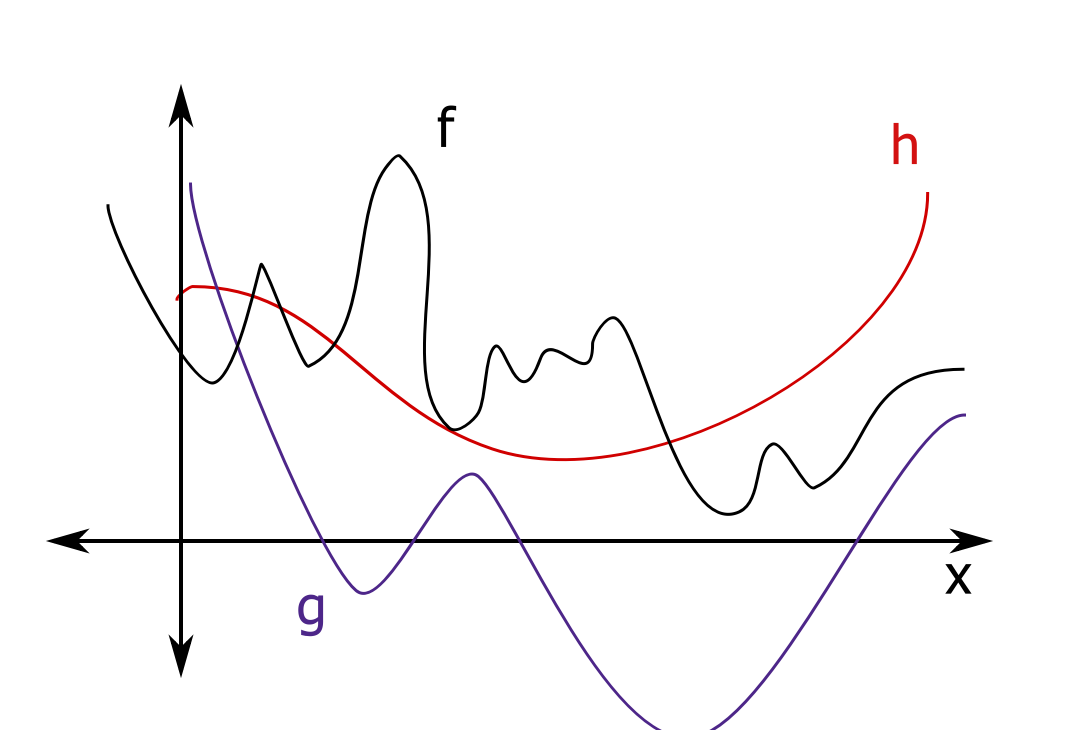
\includegraphics[width=\linewidth]{Images/optimizers.png}
    \caption{Simple and difficult objective functions to calculate a global minimizer}
    \label{fig:optimizers}
\end{figure}
\end{minipage} \vspace{15pt}

When the objective function is \textbf{smooth} or \textbf{convex}, the optimal can be found in a better way. In particular, if the function
is twice continuously differentiable, the gradients ($\nabla f$) and Hessian ($\nabla^2 f$) of the function will tell us whether $x^*$ is a local optimizer by checking some conditions. Another mathematical tool used to study smooth optimization is the Taylor’s theorem. \cite{numerical_opt}

\subsection{Inverse Problem}

\begin{minipage}{0.5\linewidth}
A good physical theory will not only describe the phenomena but also be able to make predictions about some variables of the system, if the problem is completely described by the physical model we can predict the results for some measurements of the system. This problem procedure is called a \textbf{forward problem}, it calculates the result of the model with some measured samples. While on the contrary, an \textbf{inverse problem} consists of using the outcomes of a physical model, the result, to infer the values of the parameters that characterize the physical system. The major difference between forward and inverse problem is uniqueness of the solution, while the forward problem has a unique solution, since forward problems use deterministic physical models, the inverse problem does not. \cite{inverse_problem}
\end{minipage}\hspace{20pt}
\begin{minipage}{0.45\linewidth}
\begin{figure}[H]
    \centering
    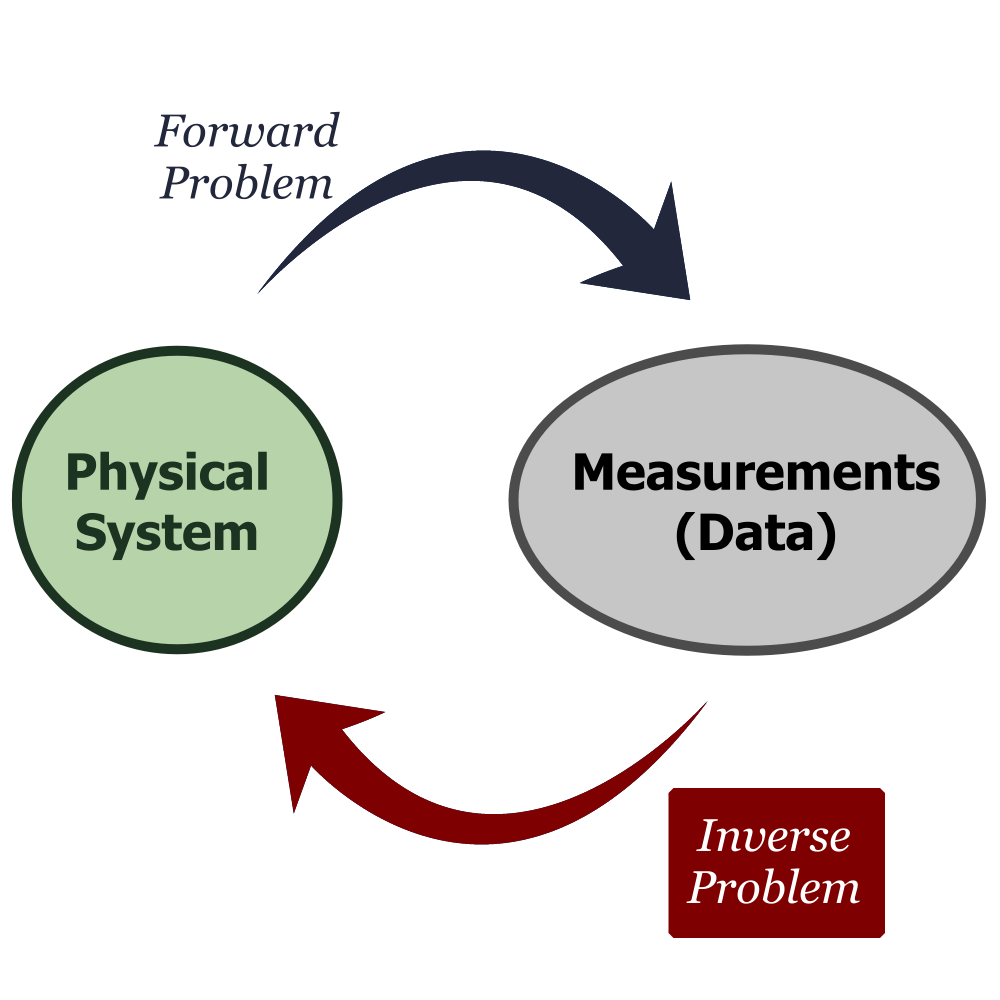
\includegraphics[width=\linewidth]{Images/invers_problem.png}
    \caption{Diagrams of inverse and forward problem.}
    \label{fig:inverse_problem}
\end{figure}
\end{minipage}
\vspace{10pt}

The notion of an inverse problem has a probabilistic nature, they are problems that involve measurements, and so a good approach is to study them on the basis of conditional probabilities and Bayes’s theorem. Another simple way to define an inverse problem is to use the probability theory: given some measurements we are interested in to find the distribution that characterizes them. \\

\textbf{Note: An inverse problem can be formulated as a minimization problem}

Let us consider the matrix equation problem $Ax=b$, with $A\in \mathbb{R}^{m\times n}$ a matrix transformation, $x\in \mathbb{R}^n$ the system variables vector, and $b\in \mathbb{R}^m$ the vector with known measured data. This is an inverse problem since we are interested in finding the system variables that best reproduce the known measured data taking into count the matrix rule transformation.\\  

The naive solution to this equation is $x=A^{-1}b$, if $A$ is well conditioned and then has an inverse, or using the Moore–Penrose inverse another solution is $x=(A^TA)^{-1}A^Tb=A^+b$. In either case the solution of this problem is to find the optimal vector $x$, that best reproduces the measurements, making use of the matrix rule transformation $A$ and the known data $b$. \\

The minimal distance is obtained when $b$ is projected onto the column space of $A$
\begin{gather*}
    b^*= Ax^*\\
    dx^* = Ax^*-b^*
\end{gather*}


\begin{minipage}{0.5\linewidth}
\begin{figure}[H]
    \centering
    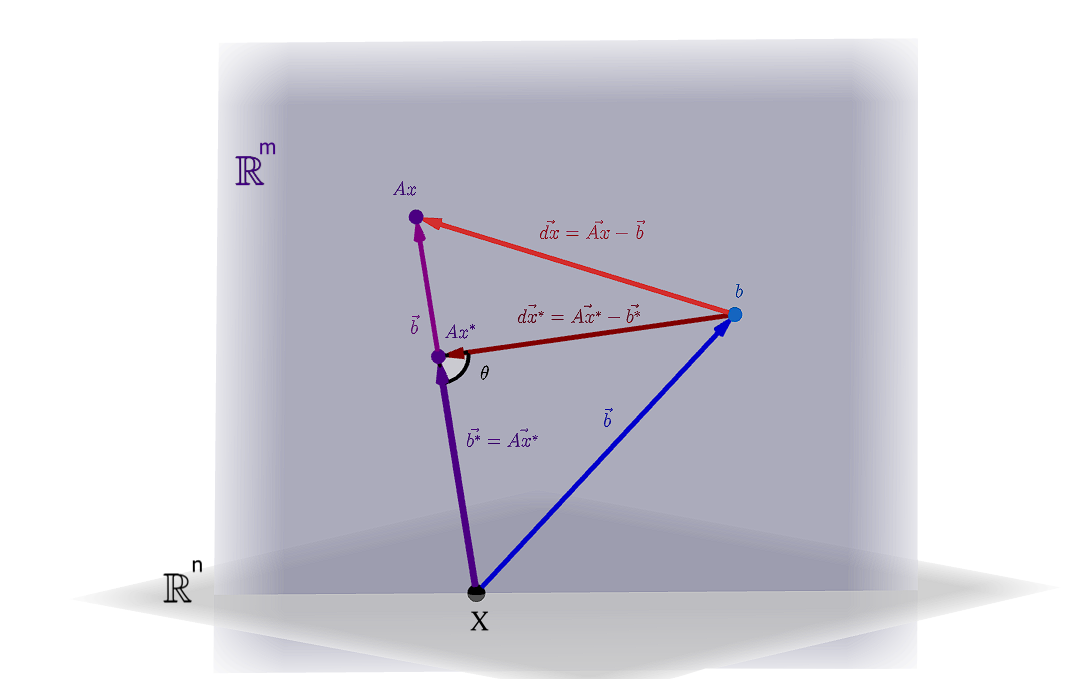
\includegraphics[width=\linewidth]{Images/linear_transformation.png}
    \caption{Linear transformation}
    \label{fig:linear_transformation}
\end{figure}
\end{minipage}\hspace{20pt}
\begin{minipage}{0.45\linewidth}

where $b$ is orthogonal to the projection $b^*$ and $Ax^*$. Therefore, $x^*$ is a solution if and only if $dx^*$ is orthogonal to the column space of $A$ 
\begin{gather*}
    A^Tdx = 0 \\ 
    A^T (Ax-b) = A^TAx-A^Tb = 0 \\
    A^TAx = A^Tb  \quad \Rightarrow \quad A = (A^TA)^{-1}A^T b
\end{gather*}
\end{minipage}

\vspace{10pt}

where again the solution is the Penrose inverse times the vector $b$ which is applicable to all least squares problems for all possibles $n$ and $m$.\\

This example shows how a linear transformation problem, an inverse problem, can be formulated as an optimization problem, minimizing the distance between two vectors, which may or may not be subject to some constraints.
\begin{align*}
    Ax = b \qquad \leftrightarrow \qquad \underset{ x \in \mathbb{R}^n}{\text{argmin}} &\quad   ||Ax-b||_2^2
\end{align*}




\subsection{Non-Linear Optimization}

The optimization literature has shown how several phenomena can be modeled with linear programming, with some good enough tolerance, but in other situations it is not sufficient. When the problem is complex to model and has a complicate objective function and constraints, linear programming is deficient and a new tool must be used, \textbf{nonlinear programming}. \textit{General nonlinear optimization} studies problems which both the objective function and functional constraints may be nonlinear functions, although the variables may have simple bounds associated. A  more formal definition of a non linear problem is the following:
\begin{equation}\label{formal_general_opt}
\begin{aligned}
\underset{ x \in \mathbb{R}^n}{\text{min}} &\quad   f(x)\\
    \text { subject to }  & \quad  \;   c_i(x)=0, \quad i \in \mathcal{E} \text {, }\\
    & \quad  \; c_j(x) \geq 0, \quad j \in \mathcal{I}\\
    & \quad  \;  l \leq x \leq u
\end{aligned}
\end{equation}

where again $f:\mathbb{R}^n \to \mathbb{R}$, $\mathcal{e}$ and $\mathcal{I}$ are the set of indices for equality and inequality constraints, respectively. The constraints are vector functions, $c_i:\mathbb{R}^n \to \mathbb{R}^m $ and $c_j:\mathbb{R}^n \to \mathbb{R}^p $ with $m=card(\mathcal{E})$ and $p=card(\mathcal{I})$, respectively. The lower bounds $l$ and upper bounds $u$ satisfies the natural conditions $-\infty < l_i \leq u_i < + \infty$ for all $i=1,\dots, n$, both bound are vectors $l,u\in \mathbb{R}^n$.\\


To guarantee solutions there are two types of optimality conditions: \textit{necessary optimality conditions} which any solution point must satisfy, and the \textit{sufficient optimality conditions} where if they are satisfied for a given point they guarantee that this point is in fact a solution. The necessary conditions are also called \textit{first order}, since they involve the gradient of the objective function and constraints. The \textbf{KKT} (Karush-Kuhn-Tucker) conditions are the cornerstones of many nonlinear optimization algorithms. Second, the \textit{second order conditions}, both necessary and sufficient, will study the second derivatives of the objective function to deduce useful information for finding the optimal point.\cite{modern_optimization}
